\section{Support-selection and refit results}
\label{app:support}
For Compact refit, a converged three-tree parent was continued along a
split-penalty path
$\lambda_s=3\cdot10^{-5},10^{-4},3\cdot10^{-4},10^{-3},3\cdot10^{-3}$,
with $\lambda_\ell=10^{-5}$. The terminal fit at the final penalty supplied
418 coefficients. Leaf-only refitting raised validation efficiency from
54.59\% to 54.81\%. Full alternating refitting converged after 15 epochs at
55.98\%; its best saved validation snapshot was epoch 8 at 56.20\%. The
selected model is this earlier snapshot, with the same 418 coefficients.
An additional one-tree oblique reference, retained in the historical uncertainty
subset but not among the final ten representatives, was trained without L1
and without SFR.

Table~\ref{tab:sfr} and Fig.~\ref{fig:tradeoff} summarize ten parent supports.
Six full refits completed, two were held for separation and two for an
inconclusive linear-program timeout. The higher-efficiency model is a completed
leaf-only refit at 57.12\%, improving its own parent by about 0.21 percentage
points. Its full stage was held and is excluded from selection. Stronger
penalization does not consistently improve the accuracy--size tradeoff;
refitting cannot restore a direction removed by support selection.

\begin{table}[htbp]\centering\small
\caption{Fixed-support refitting study. Efficiencies are percentages at 1\%
background. All models have three depth-four trees except the starred
one-tree case. Parent and leaf columns are terminal stage results; best is the
best eligible saved leaf/full refit. Held full stages contribute no candidates.
The support budget is the parent's exact nonzero count.}
\label{tab:sfr}\setlength{\tabcolsep}{4pt}
\begin{tabular}{@{}lrrrrl@{}}\toprule
$\lambda_s/\lambda_\ell$ & Support & Parent & Leaf & Best & Full stage\\\midrule
0.0001/0.0001 & 520 & 55.58 & 55.82 & 56.49 & complete \\
0.0003/1e-5 & 675 & 56.98 & 56.74 & 56.74 & timeout \\
1e-5/3e-5 & 837 & 56.91 & 57.12 & 57.12 & timeout \\
0.0003/0.0003 & 394 & 54.48 & 54.85 & 54.85 & separated \\
1e-5/1e-5$^*$ & 403 & 55.20 & 55.06 & 55.08 & complete \\
0.001/1e-5 & 561 & 56.06 & 56.32 & 56.46 & complete \\
3e-5/3e-5 & 777 & 56.62 & 56.75 & 56.75 & complete \\
1e-5/1e-5 & 889 & 56.40 & 56.45 & 56.74 & complete \\
0.003/1e-5 & 418 & 54.59 & 54.81 & 56.20 & complete \\
0.001/0.001 & 317 & 51.27 & 52.52 & 52.52 & separated \\
\bottomrule
\end{tabular}
\end{table}

\begin{figure}[H]\centering
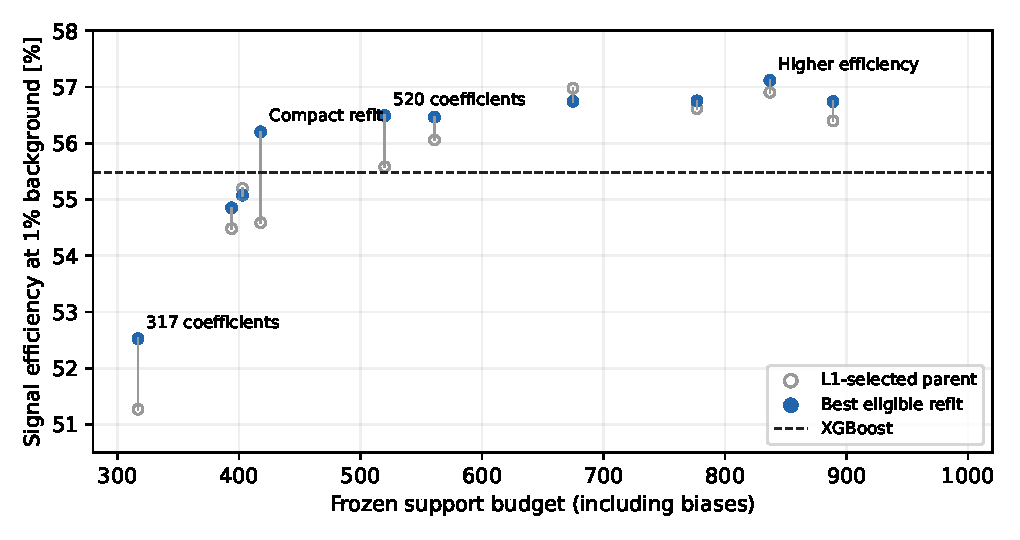
\includegraphics[width=\textwidth]{figures/sfr_research.pdf}
\caption{L1-selected terminal parents and their best eligible fixed-support
refits. Each vertical segment keeps the support budget fixed. Only refits
from eligible stages contribute; the penalty settings are given in
Table~\ref{tab:sfr}.}
\label{fig:tradeoff}
\end{figure}

\begin{implementation}
\textbf{Historical refit inputs.} This supporting study uses the v3 model bundle.
\file{fpga_handoff/CURRENT_MODEL.json} selects
\code{fpga_handoff/v3/compact_refit_3t_d4/}. The 837-coefficient alternative is
\code{highest_efficiency_3t_d4}; the one-tree reference is
\code{single_tree_1t_d4}. All exact source snapshots and masks are recorded
in the handover manifest. A later 57.24\% full-refit diagnostic for the
higher-efficiency support is held and not an eligible model.

\textbf{Compact training chain.} Start from the v2 \code{winner_3t_d4}
coefficients, run \file{configs/l1_path_v1/control.json}, then the split path
\code{split_01.json} through \code{split_05.json} in \code{configs/l1_path_v1/}.
The manifest is \file{configs/tao_l1_path_v1.json}. The final terminal parent
feeds \file{configs/support_refit_scan_v1/split300.json}. Parent training uses
\file{scripts/train_tao_fully.py}; SFR uses
\file{scripts/train_tao_support_refit.py},
\file{scripts/run_support_refit_scan_case.py} and
\file{scripts/support_refit_artifacts.py}. Exact refit reproduction begins with
the archived hash-pinned terminal parent, rather than a fresh fit at the final
penalties. The selected checkpoint hash is
\begin{center}\scriptsize\ttfamily\CompactCheckpointHash\end{center}

\textbf{Budgets.} The penalty path starts with local/joint/split iteration
budgets 300/250/300 and logs repeated chunks or adaptive increases. Compact
refit uses 400/400/800, L-BFGS-B tolerances \code{ftol=1e-12},
\code{gtol=1e-8}, at most 100 joint-fit chunks and 200 epochs per stage.
A 2,700-second allocation checkpoints with return code 75. A mild-control
router required a documented 800-to-4,000 iteration-budget amendment and
converged after 2,028 auxiliary iterations; this changed no objective or
stopping tolerances. See \file{scripts/amend_support_solver_budget.py} and
\file{docs/support_refit_scan_budget_amendments.json}.

\textbf{Snapshot layers.} The refit study was frozen on 25 October 2026.
The final comparison is separately frozen on 29 October and includes the
newly converged five-tree architecture winner at 57.73\%. Historical dated
records are retained but do not supersede this comparison.
\file{src/tao/uncertainty.py} supplies the earlier bootstrap;
\file{scripts/build_paper_inputs.py} regenerates that frozen supporting subset.
\end{implementation}
